\documentclass[12pt,a4paper]{article}
\usepackage[a4paper,margin=2.2cm]{geometry}
\usepackage{fontspec}
\usepackage{graphicx}
\usepackage{xcolor}
\usepackage{hyperref}
\usepackage{float}
\usepackage{listings}
\usepackage{array}
\usepackage{subcaption}
\usepackage{setspace}
\usepackage{titlesec}

\setmainfont{Latin Modern Roman}
\setsansfont{Latin Modern Sans}
\setmonofont{Latin Modern Mono}

\hypersetup{
  colorlinks=true,
  linkcolor=black,
  urlcolor=blue
}

\lstset{
  basicstyle=\ttfamily\small,
  frame=single,
  breaklines=true,
  showstringspaces=false,
  columns=fullflexible,
  keepspaces=true,
  numbers=left,
  numberstyle=\tiny\color{gray},
  numbersep=8pt,
  rulecolor=\color{black!15},
  backgroundcolor=\color{black!2}
}

\setstretch{1.15}
\setlength{\parskip}{6pt}
\setlength{\parindent}{0pt}
\renewcommand{\contentsname}{Icindekiler}

\titleformat{\section}{\Large\bfseries}{\thesection.}{0.5em}{}
\titleformat{\subsection}{\large\bfseries}{\thesubsection.}{0.5em}{}
\makeatletter
\renewcommand*\l@subsection{\@dottedtocline{2}{1.5em}{3.4em}}
\makeatother

\begin{document}

\tableofcontents
\clearpage

\section{Projenin Ozeti}

Bu rapor, Mobil Programlama dersi kapsaminda gelistirdigimiz \verb|kitap_kiralama| projesini anlatmak icin hazirlanmistir. Proje adinda kiralama ifadesi bulunsa da mevcut uygulama akisi kitaplari listeleyen, detayini gosteren, sepete ekleyen ve siparis gecmisini takip ettiren bir mobil arayuz uzerine kurulmustur.

Bu projede amacimiz kitap odakli bir mobil uygulama deneyimini final projesi seviyesinde duzenli, temiz ve sunulabilir bir yapiyla ortaya koymakti. Uygulama kullaniciya once kitap katalogunu sunuyor, ardindan kitap detayina inmesine izin veriyor, daha sonra sepet uzerinden siparis verme akisini tamamlatiyor. Verilen siparisler de ayri bir ekranda tutuluyor ve detayli olarak gorulebiliyor.

Projenin son surumunde uygulama yalnizca bellekte calisan bir prototip olmaktan cikarildi ve Firebase tabanli bir veri katmaniyla desteklendi. Boylece kitap katalogu Cloud Firestore uzerinden cekilmeye, kullanici girisi Firebase Authentication uzerinden yapilmaya, sepet ve siparis kayitlari da her kullaniciya ozel olarak Firestore icinde tutulmaya baslandi. Buna ek olarak yonetici paneli eklendi; admin hesabi tum siparisleri gorup kargo durumunu degistirebiliyor ve yeni kitap ekleyebiliyor.

\section{Projenin Amaci ve Kapsami}

Bu projenin temel amaci sadece bir liste ekrani gostermek degildi. Biz burada daha butunlu bir deneyim kurmak istedik:

\begin{enumerate}
  \item Kullanici uygulamayi acinca once bir oturum acma ekrani ile karsilassin.
  \item Hesabi yoksa hemen ayni ekrandan kayit olabilsin.
  \item Giris yaptiktan sonra kitaplari iki sutunlu bir duzende gorebilsin.
  \item Arama ve filtreleme ile liste icinde rahat gezebilsin.
  \item Bir kitabin detayina girip icerigi, konusu ve temel bilgilerini okuyabilsin.
  \item Begendigi kitabi sepete ekleyebilsin ve sepet veritabaninda saklansin.
  \item Siparis verince bu kayit Firestore tarafinda kalici olarak tutulsun.
  \item Gecmis siparislerden birine tiklayinca o siparisin detaylarini gorebilsin.
  \item Admin hesabi ile giris yapildiginda musteri uygulamasi yerine yonetici paneli acilsin.
  \item Yonetici tum siparisleri tek ekranda gorup kargo durumunu degistirebilsin.
  \item Yonetici yeni kitap ekleyebilsin ve magazayi onizleme modunda gezebilsin.
\end{enumerate}

Bu kapsam icinde proje, ders duzeyinde yeterli olacak kadar islevsel; ama bilincli olarak fazla karmasik olmayan bir noktada tutuldu. Yine de rapor teslim asamasinda kod yapisi daha okunur ve savunulabilir olsun diye dosya yapisi profesyonel sekilde duzenlendi ve gercek bir veri katmani eklendi.

\section{Genel Uygulama Akisi}

Uygulamanin genel akisi su sekilde ilerliyor:

\begin{enumerate}
  \item Uygulama acildiginda Firebase baslatiliyor ve oturum durumu kontrol ediliyor.
  \item Oturum yoksa giris / kayit ekrani aciliyor.
  \item Kullanici e-posta ve sifre ile giris yapiyor ya da yeni hesap olusturuyor.
  \item Giris yapan e-posta \verb|admin@gmail.com| ise yonetici paneli aciliyor.
  \item Normal kullanici girisinde ana ekranda kitap kartlari Firestore'dan cekilip listeleniyor.
  \item Ust taraftaki arama alani ile kitap, yazar veya kategori bazli arama yapabiliyor.
  \item Filtre butonu ile kategori secimi ve siralama tercihi aciliyor.
  \item Kartlardan birine tiklaninca detay sayfasi aciliyor.
  \item Detay sayfasinda kitap ozetine, neden okunmasi gerektigine ve kitap bilgilerine ulasilabiliyor.
  \item \verb|Sepete Ekle| butonu ile kitap kullanicinin Firestore sepetine kaydediliyor.
  \item \verb|Sepet| sekmesinde secilen kitaplar listeleniyor ve toplam tutar gosteriliyor.
  \item \verb|Siparis Ver| sonrasi siparis kaydi \verb|users/{uid}/orders| koleksiyonuna \verb|Onay Bekliyor| durumuyla yaziliyor ve sepet temizleniyor.
  \item Gecmis siparislerden birine tiklaninca siparis detay sayfasi aciliyor.
  \item Admin panelinde tum kullanicilarin siparisleri listeleniyor, siparis detayi acilip durum combobox ile guncelleniyor.
  \item Admin panelindeki \verb|Kitap Ekle| sekmesinden \verb|books| koleksiyonuna yeni kitap yazilabiliyor.
  \item Sag ust kosedeki cikis butonu ile oturum kapatilabiliyor.
\end{enumerate}

Bu akis teknik olarak buyuk bir e-ticaret sistemi olmasa da final projesi anlatimi icin yeterli bir butunluk sagliyor.

\section{Proje Dizin Yapisi}

Bu asamada proje yapisi daha mantikli klasorlere ayrildi ve Firebase ile ilgili dosyalar eklendi:

\begin{lstlisting}
kitap_kiralama/
|-- assets/
|   `-- covers/
|-- lib/
|   |-- app/
|   |   |-- admin_app.dart
|   |   |-- app_config.dart
|   |   `-- book_store_app.dart
|   |-- data/
|   |   |-- admin_repository.dart
|   |   |-- demo_books.dart
|   |   |-- books_repository.dart
|   |   `-- user_repository.dart
|   |-- models/
|   |   |-- book.dart
|   |   `-- order_record.dart
|   |-- screens/
|   |   |-- admin_add_book_page.dart
|   |   |-- admin_order_detail_page.dart
|   |   |-- auth_page.dart
|   |   |-- book_detail_page.dart
|   |   |-- cart_tab.dart
|   |   |-- order_detail_page.dart
|   |   |-- orders_tab.dart
|   |   `-- store_home_tab.dart
|   |-- theme/
|   |   |-- app_palette.dart
|   |   `-- app_theme.dart
|   |-- widgets/
|   |   |-- book_card.dart
|   |   |-- book_cover.dart
|   |   |-- cart_icon_badge.dart
|   |   |-- detail_info_tile.dart
|   |   |-- detail_section_card.dart
|   |   |-- detail_stat_card.dart
|   |   |-- highlight_tag.dart
|   |   |-- order_status_pill.dart
|   |   `-- summary_row.dart
|   |-- firebase_options.dart
|   `-- main.dart
|-- firestore.rules
|-- firebase.json
|-- .firebaserc
|-- reports/
|   |-- kitap_kiralama_raporu.md
|   |-- kitap_kiralama_raporu.tex
|   |-- kitap_kiralama_raporu.pdf
|   `-- screenshot_01.png ... screenshot_10.png
`-- pubspec.yaml
\end{lstlisting}

Buradaki en onemli farklar Firebase ayarlari, auth ekrani, veri repository'leri ve admin paneli dosyalarinin eklenmis olmasidir. Ayni zamanda proje koku artik \verb|firestore.rules|, \verb|firebase.json| ve \verb|.firebaserc| ile birlikte bir Firebase projesi olarak da yapilandirilmistir.

\section{Projeyi Nasil Ilerlettik}

Projeyi gelistirirken asama asama ilerledik. Ilk adimda arayuz kurgusu Figma uzerinde cizildi. Ana ekran, kitap kartlari, detay sayfasi, sepet ve alt menu yapisi once tasarim olarak netlestirildi.

Ikinci adimda bu tasarim Flutter tarafina aktarildi. Yani Figma'da dusundugumuz sayfa duzeni, renk dili ve kart yapisi Flutter widgetlari ile gercek uygulama ekranlarina donusturuldu.

Ucuncu adimda ise kullanicinin gordugu ekranlara islev kazandirildi. Bu kisimda butonlarin calismasi, menu gecisleri, kitap detayina gitme, sepete ekleme, siparis olusturma ve siparis kayitlarini listeleme gibi arka plan mantigi eklendi. Bu noktada veriler henuz yalnizca bellekte tutuluyordu.

Dorduncu adimda projeyi tek dosyali yapidan cikartip \verb|app|, \verb|screens|, \verb|models|, \verb|data|, \verb|theme| ve \verb|widgets| klasorlerine ayirdik. Boylece refactor sonrasi kod tabani daha okunabilir hale geldi.

Besinci adimda Firebase entegrasyonu yapildi. \verb|kitap-kiralama-app| adinda bir Firebase projesi olusturuldu, FlutterFire CLI ile yapilandirma dosyalari uretildi, Firestore veritabani acildi, kitap verileri Firestore'a tasindi, Authentication acilarak e-posta sifre giris destegi eklendi ve sepet ile siparisler kullanici bazli olarak Firestore icinde saklanmaya baslandi.

Son adimda ise yonetici paneli ve siparis durum yonetimi eklendi. \verb|admin@gmail.com| hesabi normal magaza yerine admin paneline yonlendirildi; admin tum siparisleri tek listede gormeye, siparis durumunu degistirmeye, yeni kitap eklemeye ve magazayi onizleme modunda gezmeye basladi.

\section{Firebase Entegrasyonu ve Veri Katmani}

Projenin son asamasinda yalnizca arayuz yeterli olmaz dusuncesiyle bir bulut veri katmani eklenmesine karar verildi. Bu kapsamda asagidaki adimlar yapildi:

\begin{enumerate}
  \item Firebase CLI uzerinden \verb|kitap-kiralama-app| projesi olusturuldu.
  \item Gerekli Firestore ve Authentication API'leri etkinlestirildi.
  \item \verb|(default)| Firestore veritabani \verb|europe-west1| bolgesinde olusturuldu.
  \item FlutterFire CLI ile \verb|lib/firebase_options.dart| dosyasi olusturularak Android, iOS ve Web icin yapilandirma uretildi.
  \item \verb|firebase_core|, \verb|firebase_auth| ve \verb|cloud_firestore| paketleri eklendi.
  \item Kitap verileri seed scripti ile Firestore'da \verb|books| koleksiyonuna yazildi.
  \item \verb|firestore.rules| dosyasi ile guvenlik kurallari yazilip Firestore'a deploy edildi.
  \item Firebase konsolundan e-posta sifre saglayicisi aktiflestirildi ve test hesabi olusturuldu.
  \item Admin hesabi icin admin kullanicisi hazirlandi.
\end{enumerate}

Firestore tarafindaki veri modeli su sekildedir:

\begin{itemize}
  \item \verb|books/{bookId}| koleksiyonu kitap dokumanlarini tutar.
  \item \verb|users/{uid}/state/cart| dokumani kullanicinin sepetindeki kitaplarin id listesini tutar.
  \item Her kullanicinin \verb|orders| alt koleksiyonu siparislerini tutar; her sipariste kod, kitap id listesi, toplam fiyat, tarih, durum, kullanici id'si ve e-posta alanlari bulunur.
\end{itemize}

Guvenlik kurallarinda kitap koleksiyonu giris yapmis kullanicilar tarafindan okunabiliyor, yazma yetkisi ise sadece admin hesabina veriliyor. Kullanici altindaki dokumanlara sahibi olan kullanici erisebiliyor. Ayrica admin, tum kullanicilarin siparislerini okuyabiliyor ve siparis durumunu guncelleyebiliyor.

\section{Kullanici Hesabi ve Oturum Yonetimi}

Uygulamada oturum yonetimi Firebase Auth akisina bakilarak yapiliyor. \verb|main.dart| icindeki kontrol; oturum yoksa \verb|AuthPage| ekranini, oturum admin hesabina aitse \verb|AdminApp| panelini, diger kullanicilarda ise \verb|BookStoreApp| kabugunu render ediyor.

\verb|AuthPage| ekrani tek bir form uzerinden hem giris hem kayit isini yapacak sekilde tasarlandi:

\begin{itemize}
  \item Kullanici "Giris Yap" modunda iken \verb|signInWithEmailAndPassword| cagrisi yapiliyor.
  \item "Kayit Ol" modunda iken \verb|createUserWithEmailAndPassword| cagrisi yapiliyor.
  \item \verb|FirebaseAuthException| durumlari yakalanip kullanici dostu bir hata mesaji olarak ekranda gosteriliyor.
\end{itemize}

Test sunumu kolay olsun diye form alanlari acilirken test hesabi bilgileriyle dolu geliyor. Uygulama icindeki cikis butonu Firebase Auth uzerinden oturumu kapatiyor.

\section{Yonetici (Admin) Paneli ve Siparis Yonetimi}

Yonetici ozellikleri sade tutuldu ve ayri bir API katmani yazilmadi. Admin hesabi olarak \verb|admin@gmail.com| kullanildi. \verb|main.dart| icindeki oturum kontrolu artik uc yonlu calisiyor: oturum yoksa giris ekrani, giris yapan kullanici admin ise admin paneli, normal kullanici ise magaza uygulamasi aciliyor.

\verb|AdminApp| uc sekmeli bir panel olarak tasarlandi:

\begin{itemize}
  \item \verb|Siparisler| sekmesi tum kullanicilarin siparislerini tek ekranda gosteriyor.
  \item \verb|Magaza| sekmesi kitap listesini admin icin onizleme modunda actiriyor.
  \item \verb|Kitap Ekle| sekmesi yeni kitap bilgilerini alip Firestore \verb|books| koleksiyonuna yaziyor.
\end{itemize}

Siparis durumu akisi onay bekliyor, hazirlaniyor, kargoya verildi ve teslim edildi adimlarindan olusuyor. Yeni verilen siparisler ilk olarak \verb|Onay Bekliyor| durumu ile kaydediliyor. Admin siparis detayina girdiginde kargo durumunu combobox ile degistirebiliyor. Bu degisiklik dogrudan ilgili kullanicinin siparis dokumanina yazildigi icin musterinin \verb|Siparislerim| ekrani da canli olarak guncelleniyor.

Tum siparisleri okumak icin admin repository icinde Firestore collection group sorgusu kullanildi. Ek indeks zorunlulugu dogmamasi icin bu sorguda \verb|orderBy| kullanilmadi; siparisler uygulama tarafinda tarihe gore yeniden eskiye siralandi.

Kitap ekleme akisinda admin kitap adi, yazar, kategori, fiyat, sayfa sayisi, alt baslik ve aciklama gibi alanlari forma giriyor. Form kaydedilince \verb|AdminRepository.addBook()| yeni dokumani \verb|books| koleksiyonuna yaziyor ve kitap listesi tekrar yukleniyor. Bu sayede eklenen kitap magazada hemen gorunuyor.

\section{Kayitlarin Saklanmasi ve Verinin Korunmasi}

Projenin ilk surumlerinde sepet ve siparis verileri sadece bellekte tutuluyordu. Son surumde bu durum tamamen degisti ve veriler Cloud Firestore uzerinden kaliciya alindi.

\begin{itemize}
  \item Kitap katalogu \verb|books| koleksiyonundan canli olarak cekiliyor.
  \item Sepet, \verb|users/{uid}/state/cart| dokumaninda tutuluyor; \verb|snapshots()| ile dinlendigi icin canli senkronize.
  \item Siparisler, kullanicinin \verb|orders| alt koleksiyonunda her siparis icin ayri bir dokuman olarak tutuluyor. Tarih, toplam tutar, kitap id listesi, durum, kullanici id'si ve kullanici e-postasi burada yer aliyor.
  \item Firestore guvenlik kurallari sayesinde her kullanici yalnizca kendi verisine erisebiliyor; admin ise sadece gerekli yonetim islemleri icin tum siparisleri okuyup durum guncelleyebiliyor.
\end{itemize}

Boylece artik uygulama kapansa, telefon yeniden baslatilsa ve hatta baska bir cihazdan giris yapilsa bile sepet ve siparis gecmisi kullanicinin yaninda kaliyor.

\section{Kullanici Deneyimi Tarafi}

Kullanici deneyiminde sade ama bos olmayan bir yapi kurmaya calistik. Bu deneyimin temeli once Figma tarafinda dusunuldu; yani kullanicinin ilk gorecegi yerlesim, arama alani, filtre butonu ve alt gezinme mantigi daha kod yazilmadan once tasarim olarak kurgulandi. Daha sonra Flutter'a aktarilan bu yapi icinde ana ekranda fazla bolum kullanmak yerine kitap listesini merkeze alan daha temiz bir yaklasim korundu. Ust kisimda sadece arama ve filtre butonu birakildi. Bu sayede kullanici ilk bakista ne yapacagini daha rahat anliyor.

Kitap detay ekranlari da sirf bir kapak ve fiyat gosteren yapida birakilmadi. Bunun yerine kitap ozeti, neden okunmasi gerektigi, kitap bilgileri ve etiketler eklenerek detay sayfasi daha dolu ve daha duzgun hale getirildi.

Siparisler tarafi da yalnizca bir liste olarak birakilmadi. Kullanici gecmis siparisine tikladiginda ayri bir detay sayfasi aciliyor ve siparisteki kitaplari tekrar gorebiliyor. Siparis durum etiketi de musteriye siparisinin hangi asamada oldugunu gosteriyor. Admin tarafinda ise tum siparisleri tek ekranda gormek ve durumu combobox ile degistirmek sunum sirasinda uygulamanin tamamlanmis bir is akisi gibi anlatilmasini sagliyor.

\section{Arayuz Tarafi}

Arayuz tarafinda klasik beyaz-mor cizgiden uzaklasmak istedik. Bu nedenle once Figma asamasinda mavi-yesil agirlikli bir tasarim dili dusunduk. Arka plan tamamen koyu degil; acik ama soguk bir ton veriyor. Kartlarda beyaz yuzeyler kullanilirken vurgu butonlari ve durum alanlarinda mavi-yesil gecisler tercih edildi. Daha sonra bu tasarim kararlari Flutter tarafinda korunarak gercek arayuze aktarildi.

Bu son duzenlemede kart yapisi da tekrar ele alindi. \verb|BookCard| bileseni ayri dosyaya tasindi ve ic yerlesimi \verb|Expanded| yapisiyla daha dayanikli hale getirildi. Grid tarafinda sabit iki sutun korunurken kart yuksekligi de buna gore ayarlandi. Yeni eklenen \verb|AuthPage| ekrani da uygulamanin geri kalan renk dilini koruyor. Admin ekranlarinda da ayni sade renk dili korundu; siparis durumu etiketleri onay bekliyor, hazirlaniyor, kargoya verildi ve teslim edildi durumlarina gore farkli renklerle gosteriliyor.

\section{Kod Bolumleri}

Asagida projede rapor acisindan en anlamli gordugumuz dosya ve kod bolumleri yer almaktadir.

\subsection{Dosya: pubspec.yaml}

\textbf{Dosyanin gorevi:} Flutter projesinin temel bagimliliklarini ve asset tanimlarini belirlemek. Bu son surumde \verb|firebase_core|, \verb|firebase_auth| ve \verb|cloud_firestore| paketleri de buraya eklendi.

\lstinputlisting[caption={pubspec.yaml}]{../pubspec.yaml}

\subsection{Dosya: lib/firebase\_options.dart}

\textbf{Dosyanin gorevi:} Android, iOS ve Web icin Firebase yapilandirmasini tek yerden saglamak.\\
\textbf{Satir sayisi:} 74

Bu dosya FlutterFire CLI tarafindan otomatik olarak uretildi. Uygulama baslarken dogru Firebase projesinin acilmasini sagliyor.

\subsection{Dosya: lib/app/app\_config.dart}

\textbf{Dosyanin gorevi:} Admin e-postasi ve siparis durum listesini tek yerde toplamak.\\
\textbf{Satir sayisi:} 13

\lstinputlisting[caption={AppConfig}]{../lib/app/app_config.dart}

Bu dosya sayesinde admin kontrolu ve durum listesi farkli ekranlarda tekrar tekrar yazilmiyor.

\subsection{Dosya: lib/main.dart}

\textbf{Dosyanin gorevi:} Firebase baslatma, uygulama tema kurulumu ve oturum durumuna gore giris ekrani / admin paneli / normal uygulama secimi.\\
\textbf{Satir sayisi:} 48

\lstinputlisting[caption={main.dart}]{../lib/main.dart}

\verb|main.dart| artik sadece Flutter calistirma gorevini degil, ayni zamanda uc yonlu oturum kontrolunu de yapiyor. Admin hesabi normal kullanici ekranina dusmeden dogrudan yonetici paneline gidiyor.

\subsection{Dosya: lib/screens/auth\_page.dart}

\textbf{Dosyanin gorevi:} Firebase Authentication uzerinden e-posta sifre ile giris ve kayit isleminin tek bir ekran uzerinden yapilmasini saglamak.\\
\textbf{Satir sayisi:} 160

\lstinputlisting[caption={AuthPage ekrani}]{../lib/screens/auth_page.dart}

Bu ekran tek bir buton ile hem giris hem kayit yapabiliyor. Form alanlari sunum icin test hesabi bilgileriyle onceden dolduruluyor.

\subsection{Dosya: lib/data/books\_repository.dart}

\textbf{Dosyanin gorevi:} Firestore icindeki \verb|books| koleksiyonundan kitaplari cekip \verb|Book| modeline donusturmek.\\
\textbf{Satir sayisi:} 46

\lstinputlisting[caption={BooksRepository}]{../lib/data/books_repository.dart}

Bu dosya artik \verb|demo_books.dart| icindeki sabit listenin yerini aliyor.

\subsection{Dosya: lib/data/user\_repository.dart}

\textbf{Dosyanin gorevi:} Giris yapmis kullanicinin sepetini ve siparis gecmisini Firestore uzerinde okumak ve yazmak.\\
\textbf{Satir sayisi:} 82

\lstinputlisting[caption={UserRepository}]{../lib/data/user_repository.dart}

Bu repository sepet icin tek bir dokuman, siparisler icin ise her siparis icin ayri bir dokuman tutar. \verb|placeOrder()| artik her yeni siparise \verb|Onay Bekliyor| durumunu, kullanici id'sini ve kullanici e-postasini da yazar. \verb|snapshots()| kullandigi icin ekranda canli olarak guncellenir.

\subsection{Dosya: lib/data/admin\_repository.dart}

\textbf{Dosyanin gorevi:} Admin panelinin tum siparisleri okumasini, siparis durumunu guncellemesini ve yeni kitap eklemesini saglamak.\\
\textbf{Satir sayisi:} 68

\lstinputlisting[caption={AdminRepository}]{../lib/data/admin_repository.dart}

Burada \verb|collectionGroup('orders')| ile tum kullanicilarin siparisleri tek akista dinleniyor. Siralama Firestore yerine uygulama tarafinda yapildigi icin ek indeks zorunlulugu olusmuyor.

\subsection{Dosya: lib/app/admin\_app.dart}

\textbf{Dosyanin gorevi:} Admin hesabiyla giris yapildiginda acilan uc sekmeli yonetici panelini kurmak.\\
\textbf{Satir sayisi:} 338

\lstinputlisting[caption={AdminApp}]{../lib/app/admin_app.dart}

\verb|AdminApp| icinde \verb|Siparisler|, \verb|Magaza| ve \verb|Kitap Ekle| sekmeleri bulunuyor. Magaza sekmesi admin icin onizleme olarak calisiyor; kitap detayinda satin alma cubugu gosterilmiyor.

\subsection{Dosya: lib/screens/admin\_order\_detail\_page.dart}

\textbf{Dosyanin gorevi:} Adminin bir siparisin kitaplarini, musteri bilgisini ve kargo durumunu ayrintili gormesini saglamak.\\
\textbf{Satir sayisi:} 287

\lstinputlisting[caption={Admin siparis detayi}]{../lib/screens/admin_order_detail_page.dart}

Bu ekranda durum combobox ile degistiriliyor. Degisiklik kaydedilince Firestore'daki siparis dokumani guncelleniyor.

\subsection{Dosya: lib/screens/admin\_add\_book\_page.dart}

\textbf{Dosyanin gorevi:} Adminin yeni kitap bilgilerini form uzerinden girip \verb|books| koleksiyonuna eklemesini saglamak.\\
\textbf{Satir sayisi:} 190

\lstinputlisting[caption={Admin kitap ekleme formu}]{../lib/screens/admin_add_book_page.dart}

Form kaydedildikten sonra kitap Firestore'a yaziliyor ve magaza listesi yeniden yukleniyor.

\subsection{Dosya: firestore.rules}

\textbf{Dosyanin gorevi:} Firestore tarafinda kimlerin neye erisecegini belirlemek.\\
\textbf{Satir sayisi:} 25

\lstinputlisting[caption={firestore.rules}]{../firestore.rules}

Kitap katalogu giris yapmis kullanicilar tarafindan okunabiliyor, kitap yazma yetkisi admin ile sinirli kaliyor. Kullanici verileri sahibine acik; admin ise tum siparisleri okuyup sadece durum guncellemesi yapabiliyor.

\subsection{Dosya: lib/app/book\_store\_app.dart}

\textbf{Dosyanin gorevi:} Uygulamanin ana sekmelerini, kitap yuklemesini, sepet ve siparis akisini ve cikis butonunu yonetmek.\\
\textbf{Satir sayisi:} 229

\lstinputlisting[caption={Uygulama kabugu}]{../lib/app/book_store_app.dart}

Bu kabuk artik kitaplari Firestore'dan cekiyor, sepet ve siparisleri repository uzerinden okuyup yaziyor. \verb|AppBar| icine eklenen cikis butonu ile oturum kapatilabiliyor.

\subsection{Dosya: lib/screens/cart\_tab.dart}

\textbf{Dosyanin gorevi:} Sepetteki urunleri listelemek, toplam tutari hesaplamak ve siparisi olusturmak.

Bu ekrandaki \verb|onPlaceOrder| cagrisi eskiden yalnizca bellege ekleme yapiyordu. Yeni surumde bu cagri \verb|BookStoreApp| icinden \verb|UserRepository.placeOrder| uzerinden Firestore'a kayit atiyor, ardindan sepet temizleniyor.

\subsection{Dosya: lib/models/order\_record.dart}

\textbf{Dosyanin gorevi:} Siparis bilgisini ekranlar ve repository'ler arasinda tasimak.\\
\textbf{Satir sayisi:} 51

\lstinputlisting[caption={OrderRecord modeli}]{../lib/models/order_record.dart}

Model artik siparis durumunu, kullanici id'sini ve kullanici e-postasini da tutuyor. Bu alanlar admin panelinde siparisi dogru kullaniciyle eslestirmek icin kullaniliyor.

\section{Sonuc ve Genel Degerlendirme}

Bu projede hedefimiz asiri buyuk bir mimari kurmak degildi. Bunun yerine final projesi seviyesinde derli toplu, duzgun gorunen ve adim adim anlatilabilecek bir kitap uygulamasi olusturduk. Geldigimiz noktada uygulama:

\begin{itemize}
  \item e-posta sifre ile giris ve kayit yapiyor,
  \item kitaplari Firestore uzerinden listeliyor,
  \item arama ve filtreleme yapiyor,
  \item detay sayfasi aciyor,
  \item sepete ekliyor ve sepeti Firestore'da saklayip canli senkronize ediyor,
  \item siparis verdiriyor ve siparisleri kullanici bazli kaydediyor,
  \item siparisleri ayri ekranda tutuyor,
  \item yonetici hesabiyla tum siparisleri tek ekranda yonetiyor,
  \item kargo durumunu onay bekliyor, hazirlaniyor, kargoya verildi ve teslim edildi adimlari arasinda degistirebiliyor,
  \item yeni kitap ekleyebiliyor,
  \item admin magazayi satin alma cubugu olmadan onizleyebiliyor,
  \item guvenlik kurallari sayesinde kullanici verisini sadece sahibine, yonetim islemlerini de admin hesabina aciyor.
\end{itemize}

Bu son duzenleme ile birlikte proje yalnizca islevsel degil, kod yapisi ve veri katmani acisindan da daha savunulabilir hale geldi. \verb|main.dart| sade bir giris noktasina indirildi; ana akis, admin paneli, ekranlar, modeller, repository'ler, ortak widgetlar ve Firebase yapilandirmasi kendi dosyalarina ayrildi. Bu haliyle proje, hem arayuz hem temel akis hem kod organizasyonu hem de bulut veri katmani acisindan tamamlanmis bir final odevi niteligindedir.

\section{Ekran Goruntuleri}

Asagidaki gorseller uygulamanin farkli ekranlarindan alinmistir.

\begin{figure}[H]
  \centering
  \begin{subfigure}[b]{0.48\textwidth}
    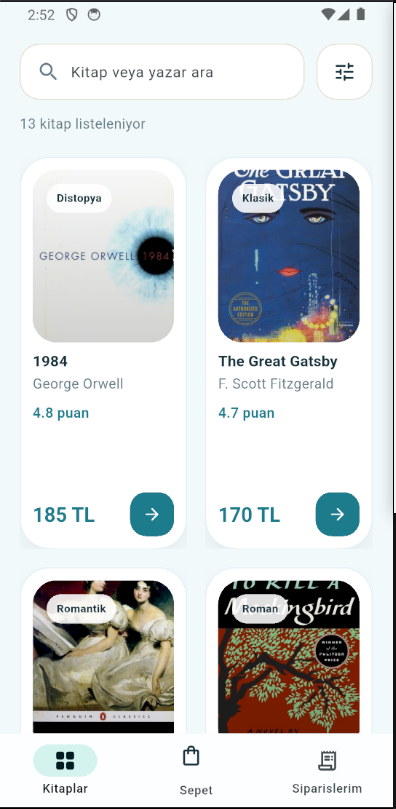
\includegraphics[width=\linewidth]{screenshot_01.png}
    \caption{Ekran goruntusu 1}
  \end{subfigure}
  \hfill
  \begin{subfigure}[b]{0.48\textwidth}
    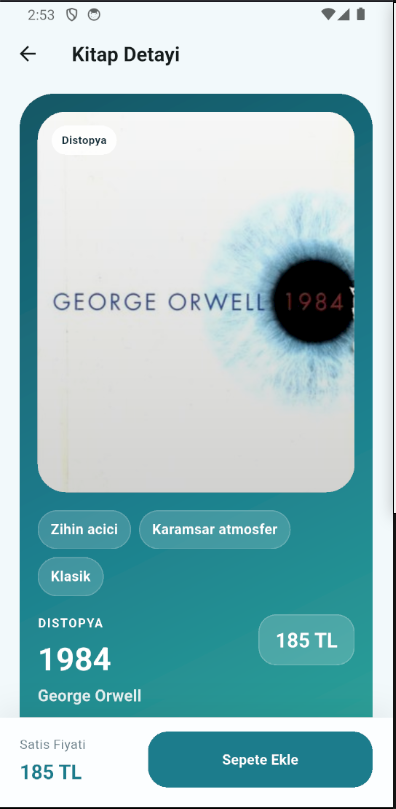
\includegraphics[width=\linewidth]{screenshot_02.png}
    \caption{Ekran goruntusu 2}
  \end{subfigure}
\end{figure}

\begin{figure}[H]
  \centering
  \begin{subfigure}[b]{0.48\textwidth}
    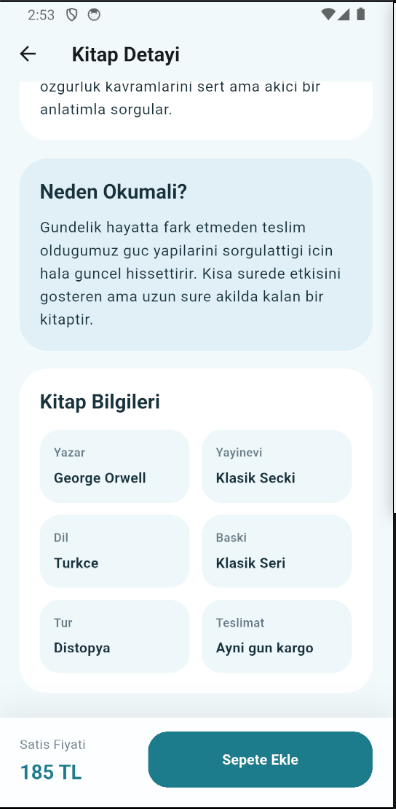
\includegraphics[width=\linewidth]{screenshot_03.png}
    \caption{Ekran goruntusu 3}
  \end{subfigure}
  \hfill
  \begin{subfigure}[b]{0.48\textwidth}
    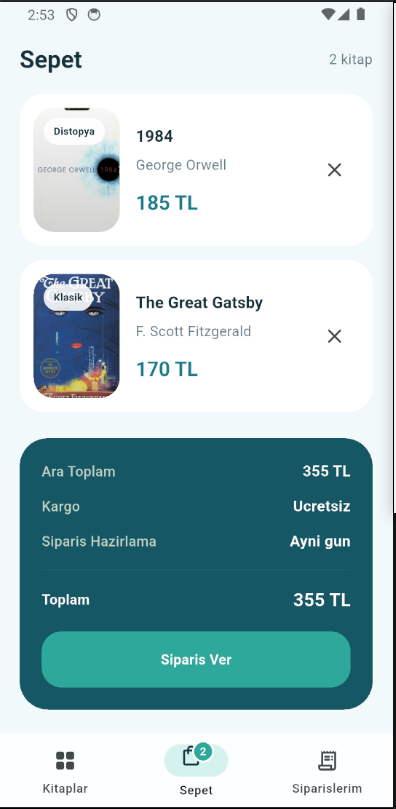
\includegraphics[width=\linewidth]{screenshot_04.png}
    \caption{Ekran goruntusu 4}
  \end{subfigure}
\end{figure}

\begin{figure}[H]
  \centering
  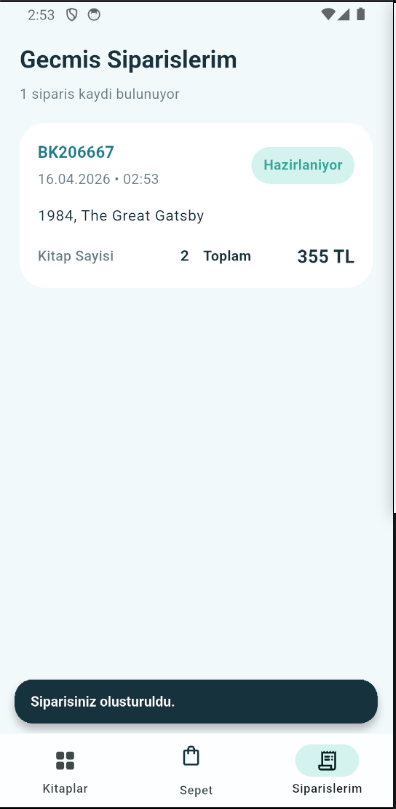
\includegraphics[width=0.55\textwidth]{screenshot_05.png}
  \caption{Ekran goruntusu 5}
\end{figure}

\begin{figure}[H]
  \centering
  \begin{subfigure}[b]{0.48\textwidth}
    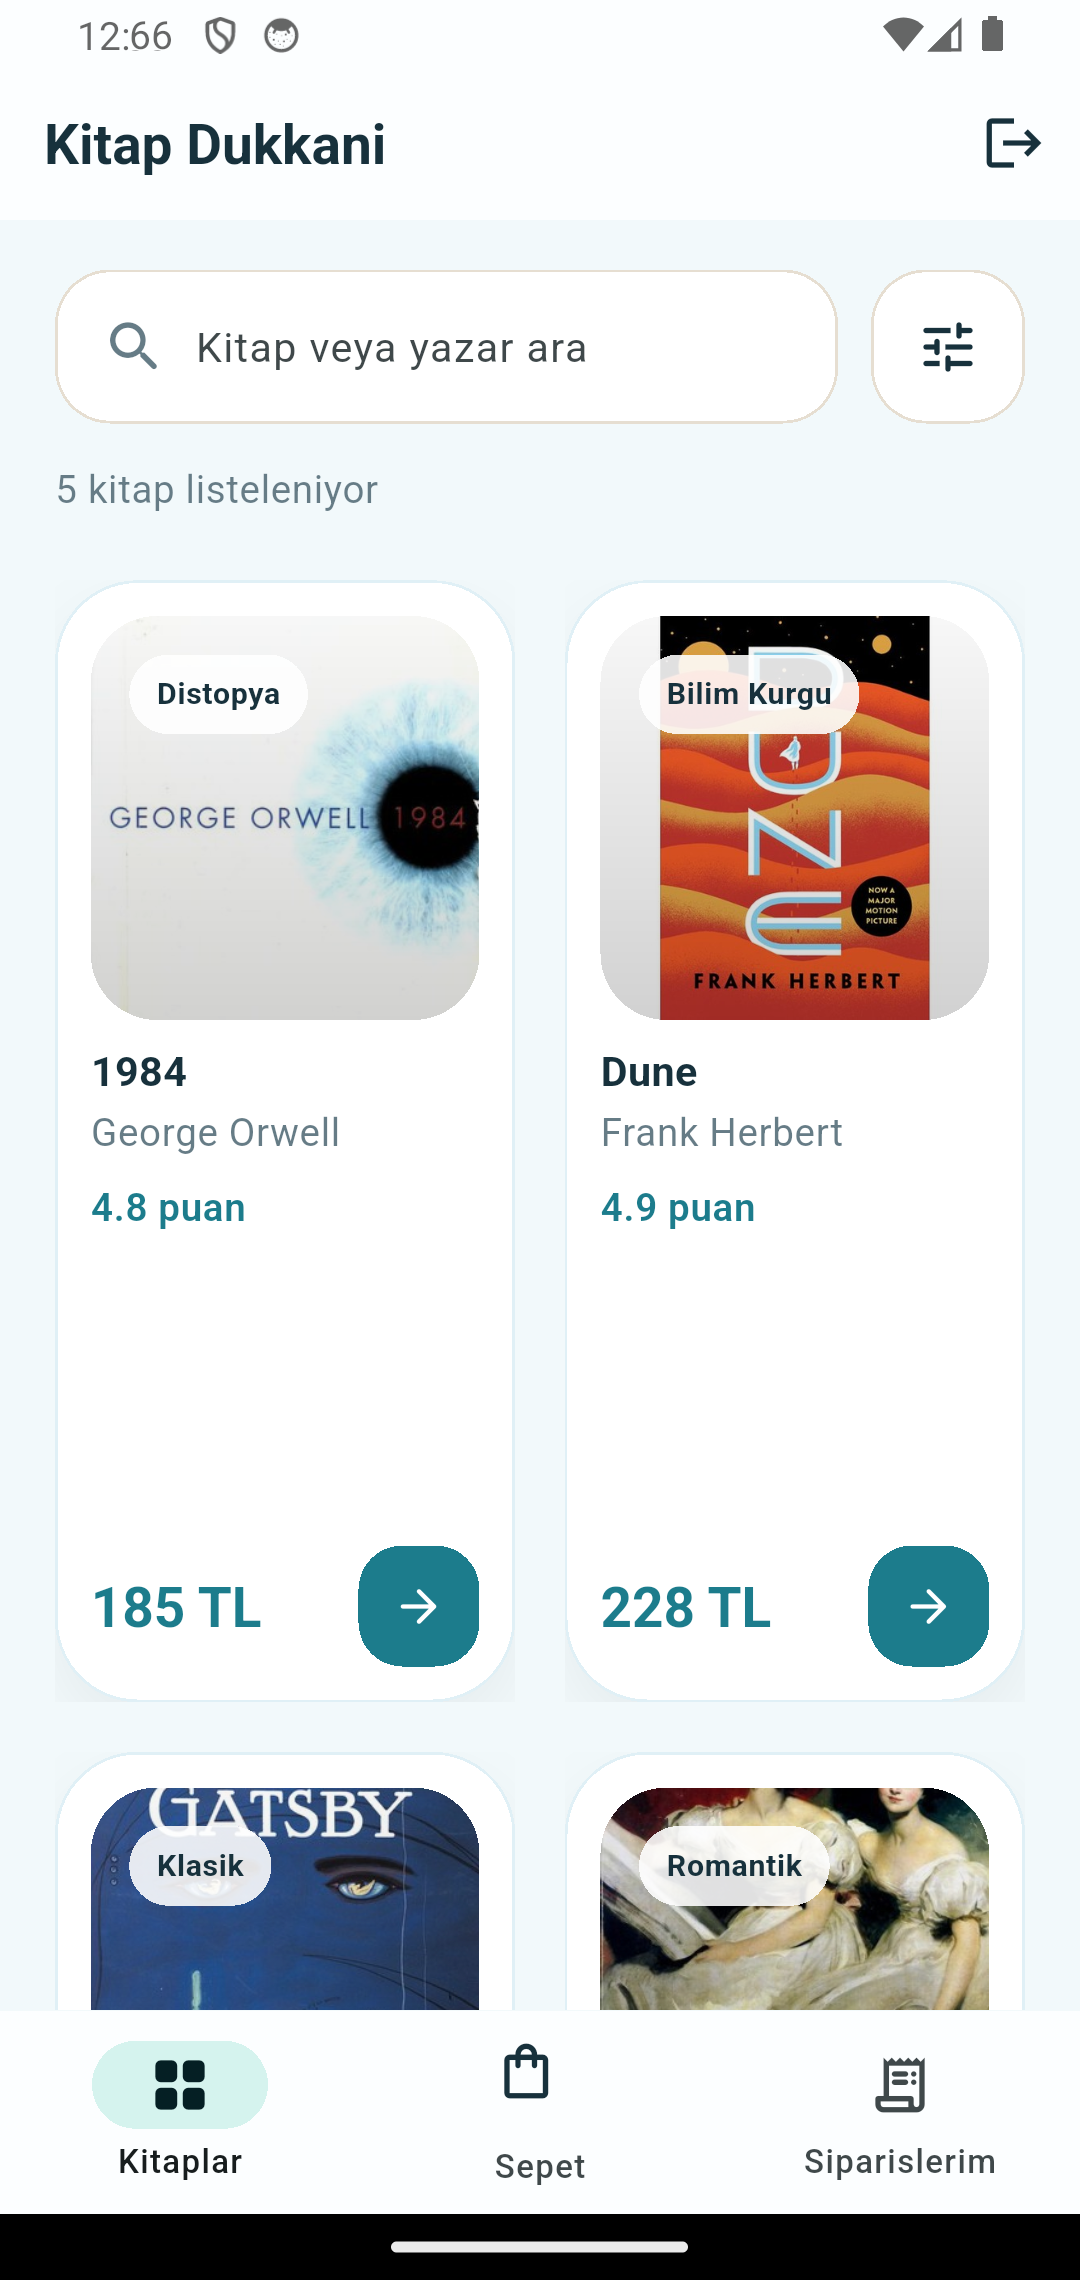
\includegraphics[width=\linewidth]{screenshot_06.png}
    \caption{Magaza ve admin onizleme}
  \end{subfigure}
  \hfill
  \begin{subfigure}[b]{0.48\textwidth}
    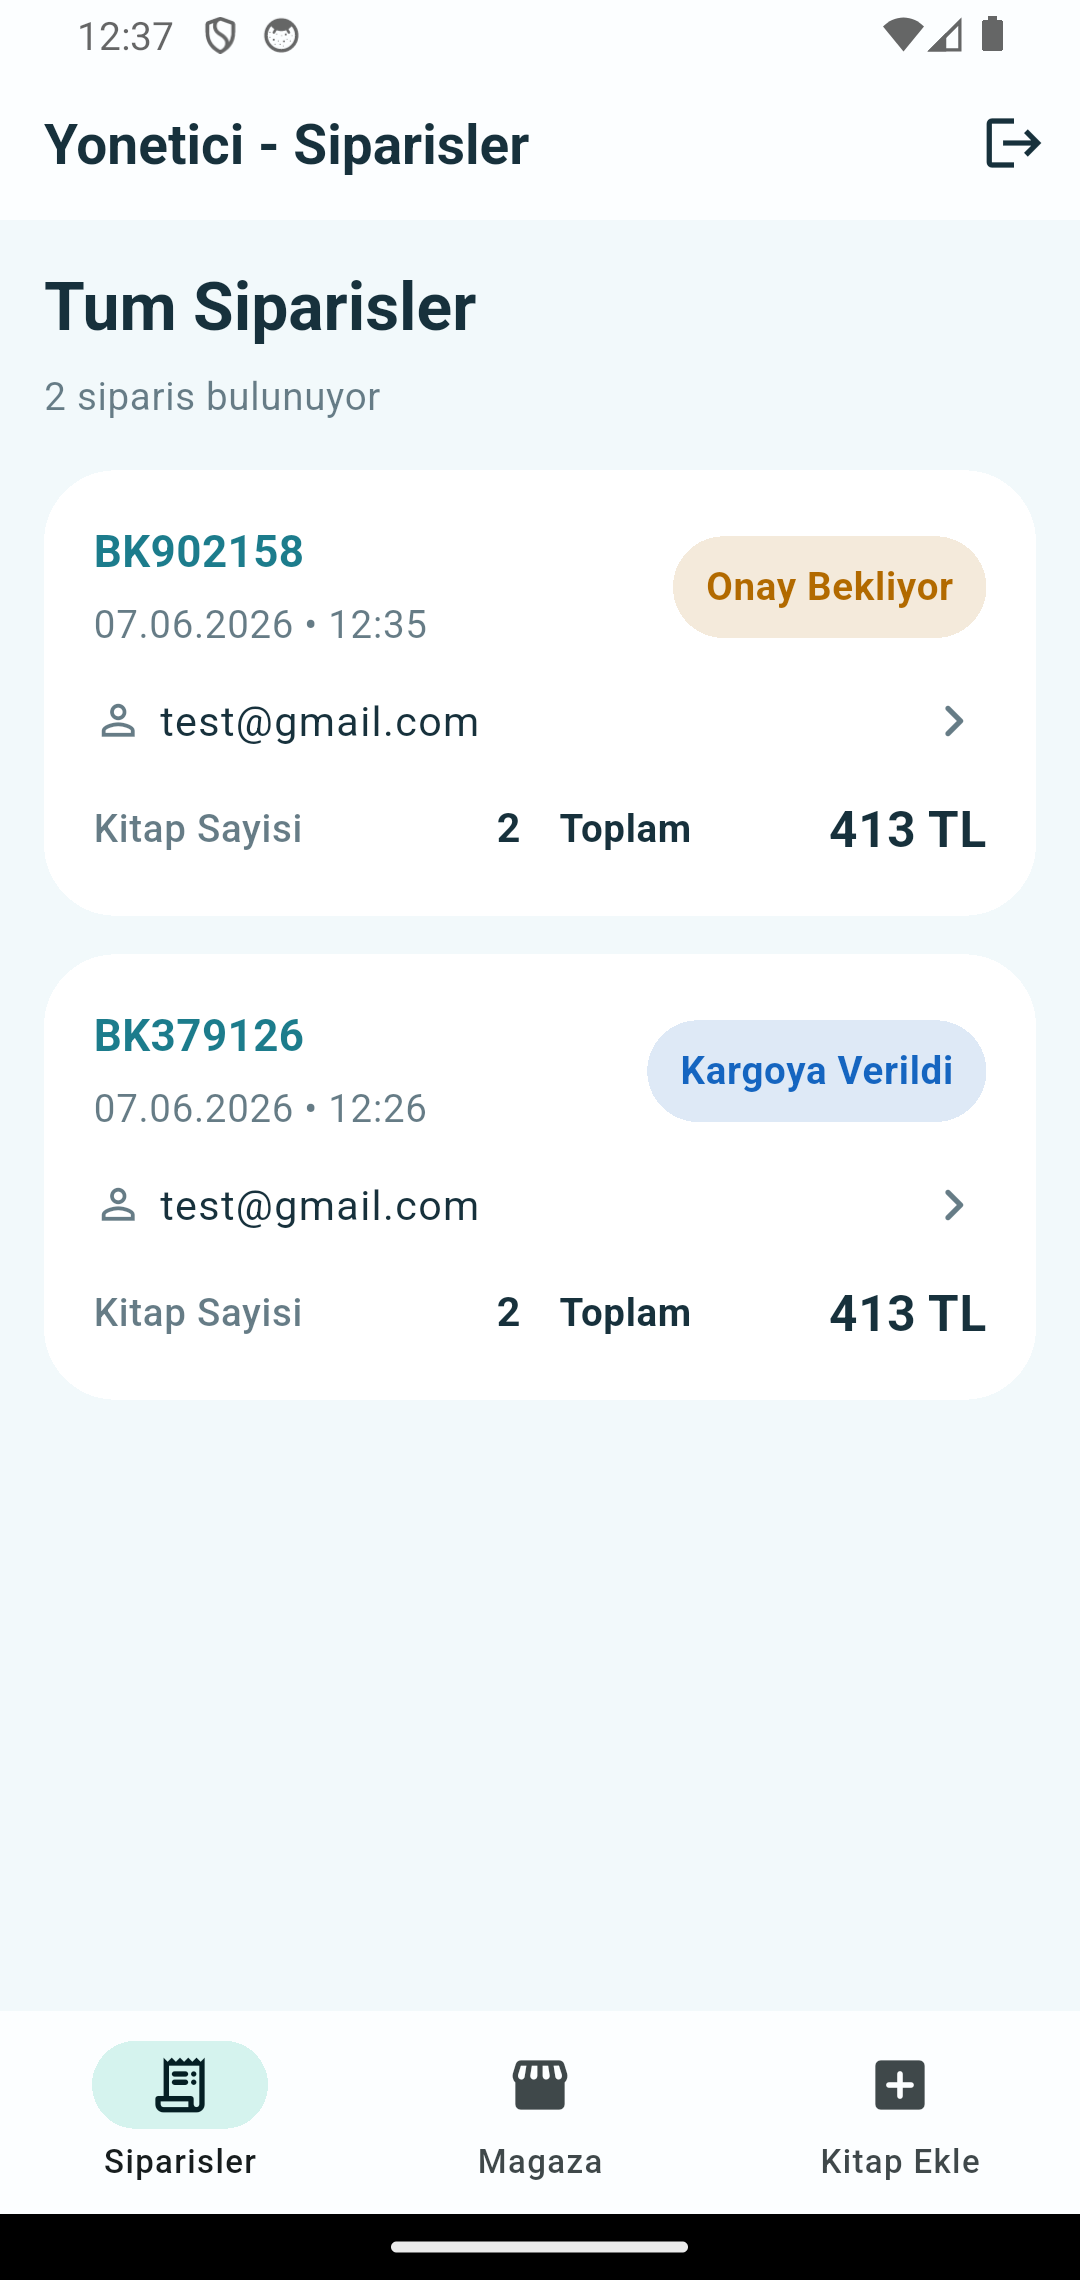
\includegraphics[width=\linewidth]{screenshot_07.png}
    \caption{Admin tum siparisler}
  \end{subfigure}
\end{figure}

\begin{figure}[H]
  \centering
  \begin{subfigure}[b]{0.48\textwidth}
    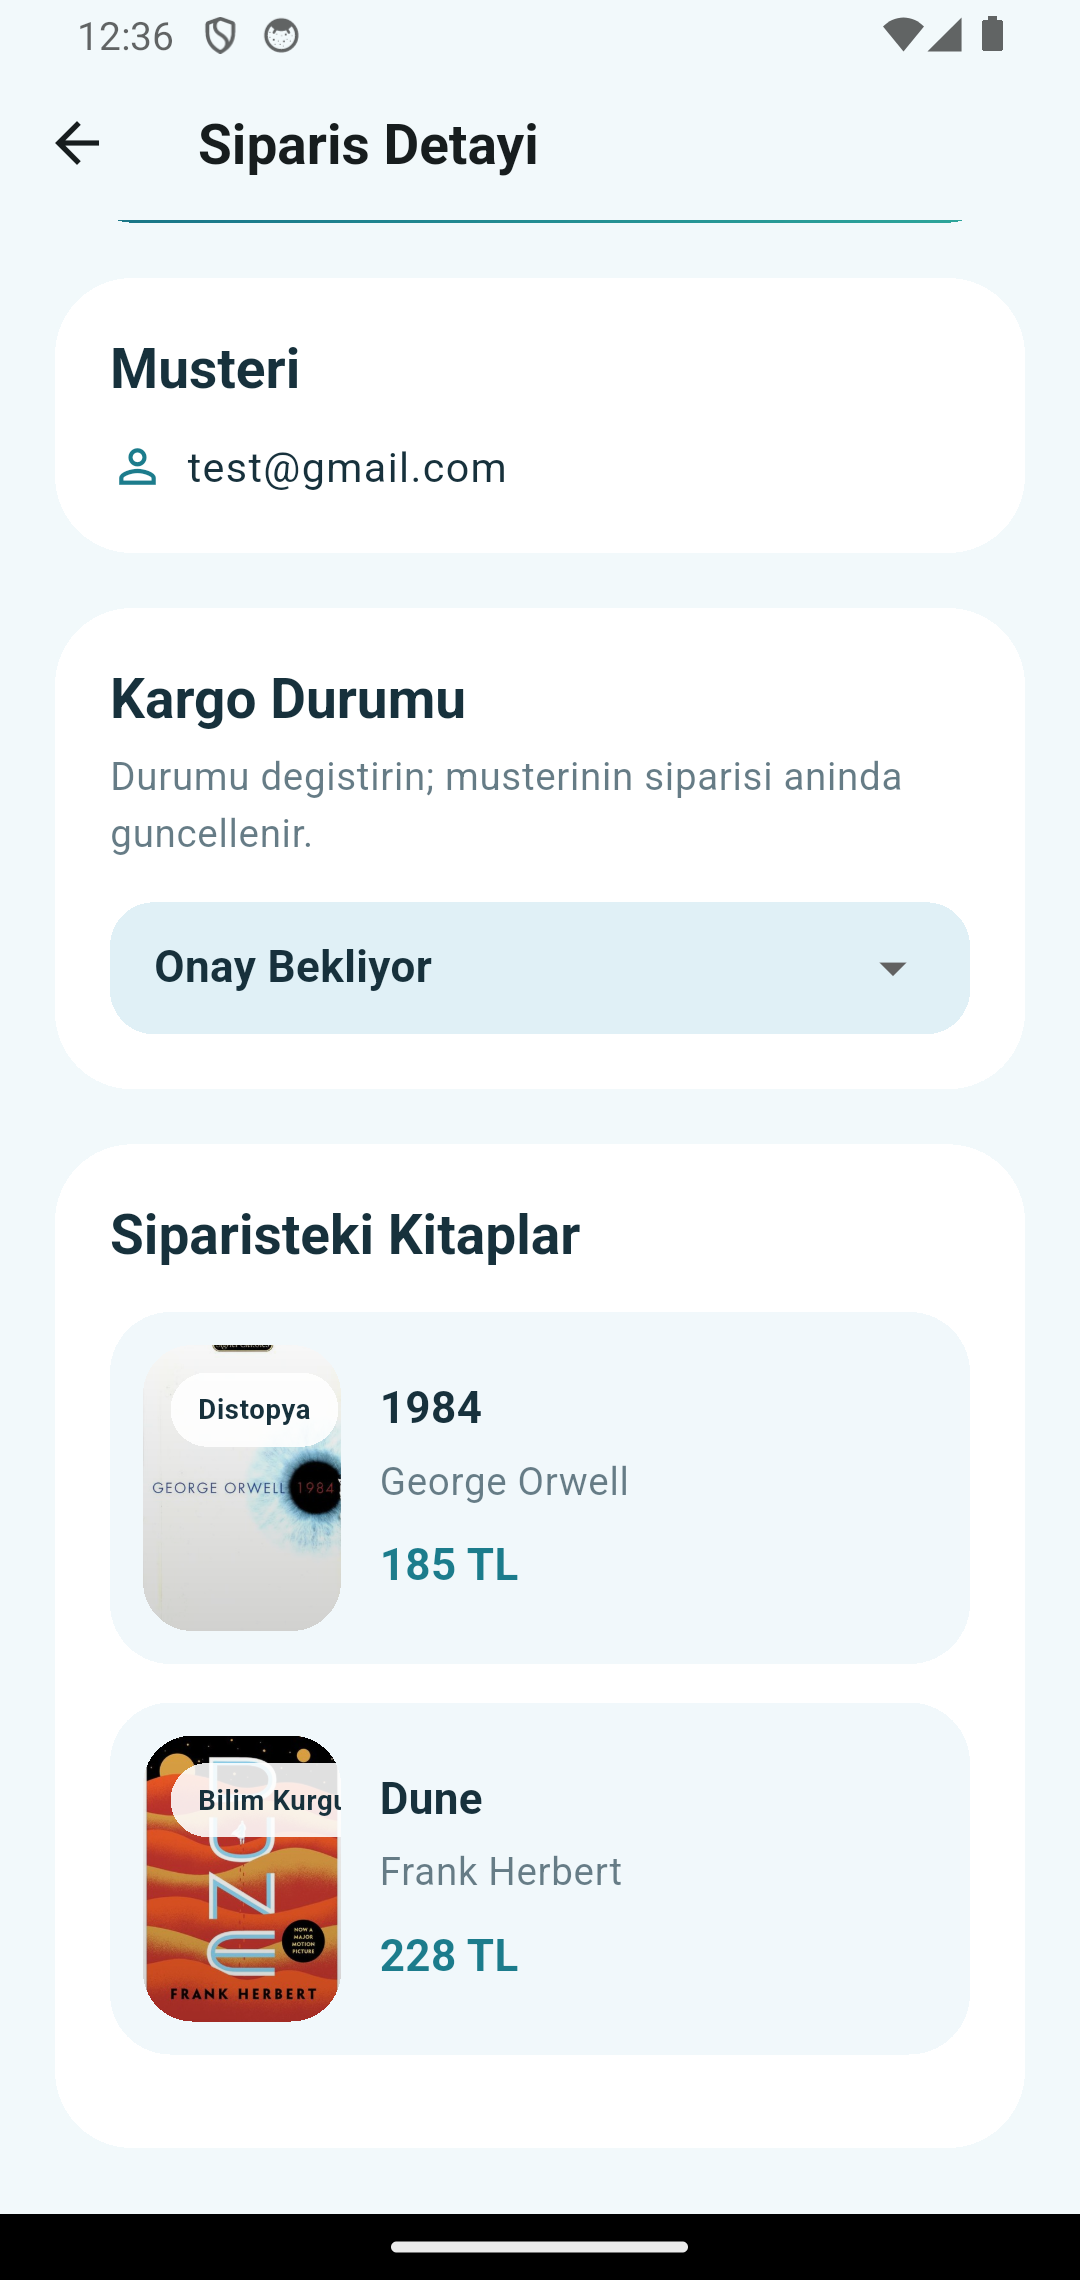
\includegraphics[width=\linewidth]{screenshot_08.png}
    \caption{Admin siparis detayi}
  \end{subfigure}
  \hfill
  \begin{subfigure}[b]{0.48\textwidth}
    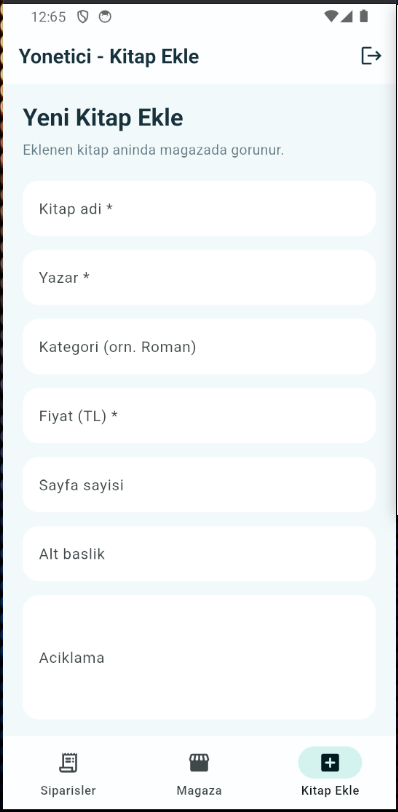
\includegraphics[width=\linewidth]{screenshot_09.png}
    \caption{Admin kitap ekleme formu}
  \end{subfigure}
\end{figure}

\begin{figure}[H]
  \centering
  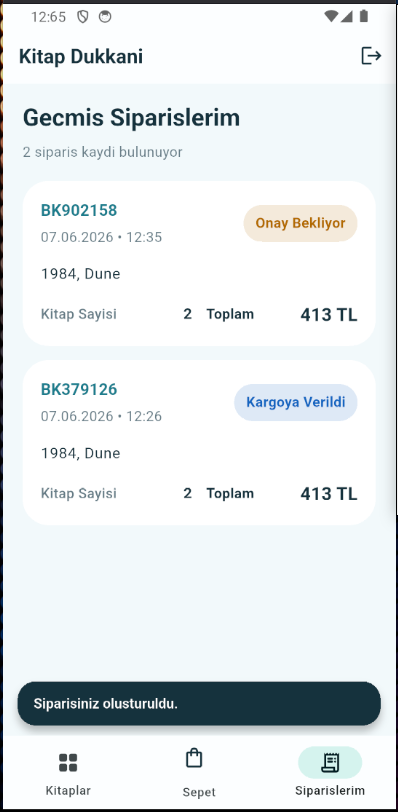
\includegraphics[width=0.55\textwidth]{screenshot_10.png}
  \caption{Musteri siparis durumlari}
\end{figure}

\end{document}
